\documentclass{beamer}
\usepackage[utf8]{inputenc}
% \usepackage[polish]{babel}
\usepackage{hyperref}
\usepackage{graphicx}
\usepackage{polski}
\usepackage[T1]{fontenc}
\usepackage{wrapfig}
\usepackage[square,numbers]{natbib}
%\bibliographystyle{unsrtnat}

\hypersetup{
    colorlinks=true,
    linkcolor=blue,
    filecolor=magenta,      
    urlcolor=cyan,
}

\usetheme{Madrid}
\usecolortheme{default}

\title [Algorytmy robotyki mobilnej]
{Algorytmy robotyki mobilnej}
\subtitle
{
    Odometria\\
}

\author[Odometria] 
{
    Wojciech Kosicki\\
    Jakub Kuśka\\
    Dawid Wilk
}
\begin{document}

\frame{\titlepage}

% \begin{frame}
% \frametitle{Plan}
% \tableofcontents
% \end{frame}

\begin{frame}{Wymiary robota}
\begin{figure}
    \centering
    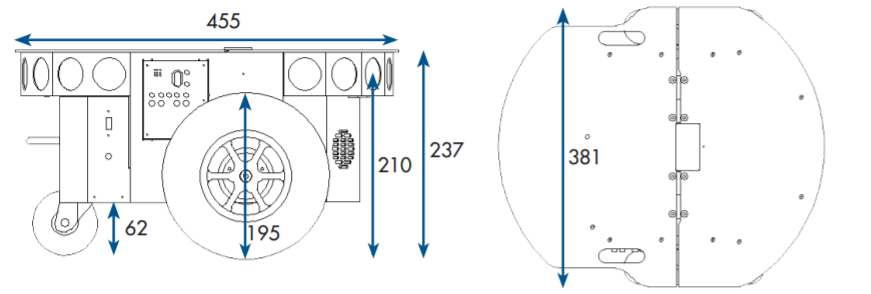
\includegraphics[width=10cm]{01.PNG}
    \caption{Wymiary robota z dokumentacji}
    \label{fig:my_label}
\end{figure}
\end{frame}

\begin{frame}{Odległość $d$ w odometrii}
\begin{figure}
    \centering
    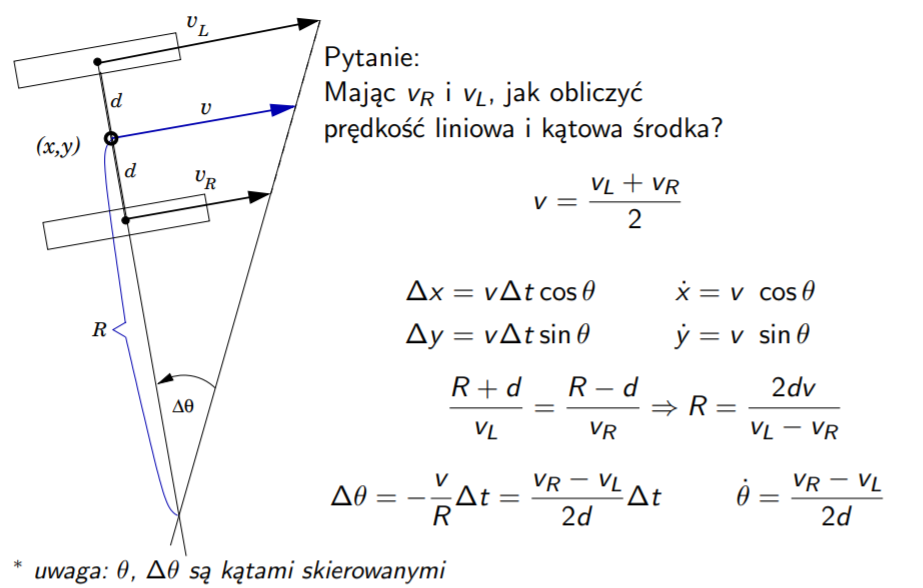
\includegraphics[width=10cm]{02.PNG}
    \caption{Wyznaczanie pozycji i orientacji robota. Slajd pochodzi z prezentacji Dra inż. Janusza Jakubiaka}
    \label{fig:my_label}
\end{figure}
\end{frame}
\begin{frame}{Badane trajektorie}
\begin{itemize} 
\item backward - opisuje ruch robota po linii prostej w tył na odległość 1.15 m,
\item forward - opisuje ruch robota po linii prostej w przódna odległość 1.15 m,
\item left full turn - opisuje obrót w miejscu robota o 360 stopni w lewo
\item right full turn - opisuje obrót w miejscu robota o 360 stopni w prawo
\item square left - ruch po kwadracie o boku 1.15 m przeciwnie do wskazówek zegara
\item square right - ruch po kwadracie o boku 1.15 m zgodnie do wskazówek zegara
\end{itemize}
\end{frame}

\begin{frame}{Uzyskane wyniki}
Przyjęta odległość między osiami obrotu kół: $d = 318mm$
\vfill
\begin{itemize}
    \item Ruch do przodu: $(x, y, \theta) = (1.13m, -0.02m, 0.01rad)$
    \begin{itemize}
        \item Błąd bezwzględny $(\Delta x, \Delta y, \Delta \theta) = (0.02m, 0.02m, 0.01rad)$
        %\item Błąd względny $(\delta x, \delta y, \delta \theta) = ()$
    \end{itemize}
    
    \item Ruch do tyłu $(x, y, \theta) = (-1.13m, 0.01m, 0.01rad)$
    \begin{itemize}
        \item Błąd bezwzględny $(\Delta x, \Delta y, \Delta \theta) = (0.02m, 0.01m, 0.01rad)$
        %\item Błąd względny $(\delta x, \delta y, \delta \theta) = ()$ 
    \end{itemize}
    
    \item Pełen obrót w lewo $(x, y, \theta) = (0.01m, -0.2m, 6.30rad)$
    \begin{itemize}
        \item Błąd bezwzględny $(\Delta x, \Delta y, \Delta \theta) = (0.01m, 0.2m, 0.02rad)$
        %\item Błąd względny $(\delta x, \delta y, \delta \theta) = ()$
    \end{itemize}
    
    \item Pełen obrót w prawo $(x, y, \theta) = (0.04m, -0.01m, -6.29rad)$
    \begin{itemize}
        \item Błąd bezwzględny $(\Delta x, \Delta y, \Delta \theta) = (0.04m, 0.01m, 0.01rad)$
        %\item Błąd względny $(\delta x, \delta y, \delta \theta) = ()$
    \end{itemize}
\end{itemize}
    
\end{frame}
\begin{frame}{Uzyskane wyniki}

\begin{itemize}
    \item Ruch po kwadracie w lewo: $(x, y, \theta) = (0.08m, -0.05m, 6.32rad)$
    \begin{itemize}
        \item Błąd bezwzględny $(\Delta x, \Delta y, \Delta \theta) = (0.08m, 0.05m, 0.04rad)$
        %\item Błąd względny $(\delta x, \delta y, \delta \theta) = ()$
    \end{itemize}
    
    \item Ruch po kwadracie w prawo: $(x, y, \theta) = (0.01m, -0.03m, -6.33rad)$
    \begin{itemize}
        \item Błąd bezwzględny $(\Delta x, \Delta y, \Delta \theta) = (0.01m, 0.03m, 0.05rad)$
        %\item Błąd względny $(\delta x, \delta y, \delta \theta) = ()$
    \end{itemize}
    
\end{itemize}
\end{frame}
\begin{frame}{Przykładowe Trajektorie}
\begin{columns}
 
\column{0.5\textwidth}
\begin{figure}[ht]
    \centering
    \includegraphics[width=6.5cm]{circleleft.png}
    \caption{Obrót w lewo}
\end{figure}

 
\column{0.5\textwidth}
\begin{figure}[ht]
    \centering
    \includegraphics[width=6.5cm]{sqright.png}
    \caption{Ruch po kwadracie w prawo}
\end{figure}

\end{columns}
\end{frame}
\end{document}

